\appendix
\section*{Appendix}

\section{Multihead Self-attention}
\label{sec:self_attention}
Standard $\mbf{qkv}$ self-attention (SA, \citet{vaswani2017}) is a popular building block for neural architectures. For each element in an input sequence $\mbf{z} \in \mathbb{R}^{N \times D}$, we compute a weighted sum over all values $\mbf{v}$ in the sequence. The attention weights $A_{ij}$ are based on the pairwise similarity between two elements of the sequence and their respective query $\mbf{q}^i$ and key $\mbf{k}^j$ representations.
\begin{align}
    [\mbf{q}, \mbf{k}, \mbf{v}] &= \mbf{z} \mbf{U}_{qkv}
    & \mbf{U}_{qkv} &\in \mathbb{R}^{D \times 3 D_h} , \label{eq:qkv} \\
    A &= \op{softmax}\left(\mbf{q}\mbf{k}^\top / \sqrt{D_h}\right)
    & A &\in \mathbb{R}^{N \times N} , \label{eq:attn_matrix}\\
    \op{SA}(\mbf{z}) &= A\mbf{v}\,. \label{eq:selfattn}
\end{align}

Multihead self-attention (MSA) is an extension of SA in which we run $k$ self-attention operations, called ``heads'', in parallel, and project their concatenated outputs. To keep compute and number of parameters constant when changing $k$, $D_h$ (Eq.~\ref{eq:qkv}) is typically set to $D/k$.
\begin{align}
    \op{MSA}(\mbf{z}) &= [\op{SA}_1(z); \op{SA}_2(z); \cdots ; \op{SA}_k(z)] \, \mbf{U}_{msa} & \mbf{U}_{msa} \in \mathbb{R}^{k \cdot D_h \times D} \label{eq:msa}
\end{align}

\section{Experiment details}

\subsection{Training}\label{sec:training}
\begin{table}[t]
\centering
\small
\begin{tabular}{l l c c c c c c c}
\toprule
Models & Dataset & Epochs & Base LR & LR decay & Weight decay  & Dropout\\
\midrule
\oursabbrv-B/\{16,32\}     & JFT-300M     & 7     & $8 \cdot 10^{-4}$ & linear & 0.1  & 0.0 \\
\oursabbrv-L/32            & JFT-300M     & 7     & $6 \cdot 10^{-4}$ & linear & 0.1  & 0.0 \\
\oursabbrv-L/16            & JFT-300M     & 7/14  & $4 \cdot 10^{-4}$ & linear & 0.1  & 0.0 \\
\oursabbrv-H/14            & JFT-300M     & 14    & $3 \cdot 10^{-4}$ & linear & 0.1  & 0.0 \\
R50x\{1,2\}                & JFT-300M     & 7     & $10^{-3}$         & linear & 0.1  & 0.0 \\
R101x1                     & JFT-300M     & 7     & $8 \cdot 10^{-4}$ & linear & 0.1  & 0.0 \\
R152x\{1,2\}               & JFT-300M     & 7     & $6 \cdot 10^{-4}$ & linear & 0.1  & 0.0 \\
R50+\oursabbrv-B/\{16,32\} & JFT-300M     & 7     & $8 \cdot 10^{-4}$ & linear & 0.1  & 0.0 \\
R50+\oursabbrv-L/32        & JFT-300M     & 7     & $2 \cdot 10^{-4}$ & linear & 0.1  & 0.0 \\
R50+\oursabbrv-L/16        & JFT-300M     & 7/14  & $4 \cdot 10^{-4}$ & linear & 0.1  & 0.0 \\
\oursabbrv-B/\{16,32\}     & ImageNet-21k & 90    & $10^{-3}$         & linear & 0.03 & 0.1 \\
\oursabbrv-L/\{16,32\}     & ImageNet-21k & 30/90 & $10^{-3}$         & linear & 0.03 & 0.1 \\
\oursabbrv-$\ast$          & \imagenet    & 300   & $3 \cdot 10^{-3}$ & cosine & 0.3  & 0.1 \\
\bottomrule
\end{tabular}
\caption{Hyperparameters for training. All models are trained with a batch size of 4096 and learning rate warmup of 10k steps. For \imagenet we found it beneficial to additionally apply gradient clipping at global norm 1. Training resolution is 224.}
\label{tbl:hparams-training}
\end{table}

Table~\ref{tbl:hparams-training} summarizes our training setups for our different models. We found strong regularization to be key when training models from scratch on \imagenet. Dropout, when used, is applied after every dense layer except for the the qkv-projections and directly after adding positional- to patch embeddings. Hybrid models are trained with the exact setup as their \oursabbrv counterparts. Finally, all training is done on resolution 224.



\subsubsection{Fine-tuning}\label{sec:finetuning}


\begin{table}[t]
\centering
\small
\begin{tabular}{l c c}
\toprule
Dataset            & Steps               & Base LR                      \\
\midrule
\imagenet           & 20\,000             & \{0.003, 0.01, 0.03, 0.06\}  \\
CIFAR100           & 10\,000             & \{0.001, 0.003, 0.01, 0.03\} \\
CIFAR10            & 10\,000             & \{0.001, 0.003, 0.01, 0.03\} \\
Oxford-IIIT Pets   & 500                 & \{0.001, 0.003, 0.01, 0.03\} \\
Oxford Flowers-102 & 500                 & \{0.001, 0.003, 0.01, 0.03\} \\
VTAB (19 tasks)    & 2\,500 & 0.01                                      \\
\bottomrule
\end{tabular}
\caption{Hyperparameters for fine-tuning. All models are fine-tuned with cosine learning rate decay, a batch size of 512, no weight decay, and grad clipping at global norm 1. If not mentioned otherwise, fine-tuning resolution is 384.}
\label{tbl:hparams-finetuning}
\end{table}


We fine-tune all \oursabbrv models using SGD with a momentum of 0.9.
We run a small grid search over learning rates, see learning rate ranges in Table~\ref{tbl:hparams-finetuning}. To do so, we use small sub-splits from the training set (10\% for Pets and Flowers, 2\% for CIFAR, 1\% \imagenet) as development set and train on the remaining data. For final results we train on the entire training set and evaluate on the respective test data.
For fine-tuning ResNets and hybrid models we use the exact same setup, with the only exception of \imagenet where we add another value $0.06$ to the learning rate sweep.
Additionally, for ResNets we also run the setup of \citet{kolesnikov2020-bit} and select the best results across this run and our sweep.
Finally, if not mentioned otherwise, all fine-tuning experiments run at 384 resolution (running fine-tuning at different resolution than training is common practice \citep{kolesnikov2020-bit}).

When transferring ViT models to another dataset, we remove the whole head (two linear layers) and replace it by a single, zero-initialized linear layer outputting the number of classes required by the target dataset.
We found this to be a little more robust than simply re-initializing the very last layer.

For VTAB we follow the protocol in~\citet{kolesnikov2020-bit}, and use the same hyperparameter setting for all tasks.
We use a learning rate of $0.01$ and train for $2500$ steps (Tab.~\ref{tbl:hparams-finetuning}).
We chose this setting by running a small sweep over two learning rates and two schedules, and selecting the setting with the highest VTAB score on the 200-example validation sets.
We follow the pre-processing used in~\cite{kolesnikov2020-bit}, except that we do not use task-specific input resolutions.
Instead we find that \oursfull{} benefits most from a high resolution ($384\times 384$) for all tasks.

\subsubsection{Self-supervision}\label{sec:self_supervision}

We employ the \textit{masked patch prediction} objective for preliminary self-supervision experiments. To do so we corrupt 50\% of patch embeddings by either replacing their embeddings with a learnable \verb|[mask]| embedding (80\%), a random other patch embedding (10\%) or just keeping them as is (10\%). This setup is very similar to the one used for language by \citet{devlin19-bert}. Finally, we predict the 3-bit, mean color (i.e., 512 colors in total) of every corrupted patch using their respective patch representations.

We trained our self-supervised model for 1M steps (ca. 14 epochs) with batch size 4096 on JFT. We use Adam, with a base learning rate of $2 \cdot 10^{-4}$, warmup of 10k steps and cosine learning rate decay. As prediction targets for pretraining we tried the following settings: 1) predicting only the mean, 3bit color (i.e., 1 prediction of 512 colors), 2) predicting a $4 \times 4$ downsized version of the $16 \times 16$ patch with 3bit colors in parallel (i.e., 16 predictions of 512 colors), 3) regression on the full patch using L2 (i.e., 256 regressions on the 3 RGB channels). Surprisingly, we found that all worked quite well, though L2 was slightly worse. We report final results only for option 1) because it has shown best few-shot performance. We also experimented with 15\% corruption rate as used by \citet{devlin19-bert} but results were also slightly worse on our few-shot metrics.

Lastly, we would like to remark that our instantiation of masked patch prediction doesn't require such an enormous amount of pretraining nor a large dataset such as JFT in order to lead to similar performance gains on ImageNet classification. That is, we observed diminishing returns on downstream performance after 100k pretraining steps, and see similar gains when pretraining on ImageNet.

\section{Additional Results}

We report detailed results corresponding to the figures presented in the paper.
Table~\ref{tbl:imagenet_imagenet21k_jft} corresponds to Figure~\ref{fig:imagenet_imagenet21k_jft} from the paper and shows transfer performance of different \oursabbrv models pre-trained on datasets of increasing size: ImageNet, ImageNet-21k, and JFT-300M.
Table~\ref{tbl:scaling_architectures} corresponds to Figure~\ref{fig:scaling_architectures} from the paper and shows the transfer performance of \oursabbrv{}, ResNet, and hybrid models of varying size, as well as the estimated computational cost of their pre-training.

\begin{table}[]
\resizebox{1.0\textwidth}{!}{
\centering
\begin{tabular}{llrrrrl}
\toprule
         &                  &  ViT-B/16 &  ViT-B/32 &  ViT-L/16 &  ViT-L/32 & ViT-H/14 \\
\midrule
\imagenet & CIFAR-10 &     98.13 &     97.77 &     97.86 &     97.94 &        - \\
         & CIFAR-100 &     87.13 &     86.31 &     86.35 &     87.07 &        - \\
         & \imagenet &     77.91 &     73.38 &     76.53 &     71.16 &        - \\
         & \imagenet ReaL &     83.57 &     79.56 &     82.19 &     77.83 &        - \\
         & Oxford Flowers-102 &     89.49 &     85.43 &     89.66 &     86.36 &        - \\
         & Oxford-IIIT-Pets &     93.81 &     92.04 &     93.64 &     91.35 &        - \\
\midrule
ImageNet-21k & CIFAR-10 &     98.95 &     98.79 &     99.16 &     99.13 &    99.27 \\
         & CIFAR-100 &     91.67 &     91.97 &     93.44 &     93.04 &    93.82 \\
         & \imagenet &     83.97 &     81.28 &     85.15 &     80.99 &    85.13 \\
         & \imagenet ReaL &     88.35 &     86.63 &     88.40 &     85.65 &    88.70 \\
         & Oxford Flowers-102 &     99.38 &     99.11 &     99.61 &     99.19 &    99.51 \\
         & Oxford-IIIT-Pets &     94.43 &     93.02 &     94.73 &     93.09 &    94.82 \\
\midrule
JFT-300M & CIFAR-10 &     99.00 &     98.61 &     99.38 &     99.19 &    99.50 \\
         & CIFAR-100 &     91.87 &     90.49 &     94.04 &     92.52 &    94.55 \\
         & \imagenet &     84.15 &     80.73 &     87.12 &     84.37 &    88.04 \\
         & \imagenet ReaL &     88.85 &     86.27 &     89.99 &     88.28 &    90.33 \\
         & Oxford Flowers-102 &     99.56 &     99.27 &     99.56 &     99.45 &   99.68 \\
         & Oxford-IIIT-Pets &     95.80 &     93.40 &     97.11 &     95.83 &     97.56 \\
\bottomrule
\end{tabular}}
\caption{Top1 accuracy (in \%) of \oursfull on various datasets when pre-trained on \imagenet, ImageNet-21k or JFT300M. These values correspond to Figure~\ref{fig:imagenet_imagenet21k_jft} in the main text. Models are fine-tuned at 384 resolution. Note that the ImageNet results are computed without additional techniques (Polyak averaging and 512 resolution images) used to achieve results in Table~\ref{tbl:best_results}.}
\label{tbl:imagenet_imagenet21k_jft}
\end{table}

\begin{table}[]
\resizebox{1.0\textwidth}{!}{
\centering
\begin{tabular}{llccccccc}
\toprule
{} &  Epochs &  ImageNet &  ImageNet ReaL &  CIFAR-10 &  CIFAR-100 &  Pets &  Flowers &  exaFLOPs \\
name           &         &           &                &           &            &       &          &           \\
\midrule
ViT-B/32       &       7 &     80.73 &          86.27 &     98.61 &      90.49 & 93.40 &    99.27 &        55 \\
ViT-B/16       &       7 &     84.15 &          88.85 &     99.00 &      91.87 & 95.80 &    99.56 &       224 \\
ViT-L/32       &       7 &     84.37 &          88.28 &     99.19 &      92.52 & 95.83 &    99.45 &       196 \\
ViT-L/16       &       7 &     86.30 &          89.43 &     99.38 &      93.46 & 96.81 &    99.66 &       783 \\
ViT-L/16       &      14 &     87.12 &          89.99 &     99.38 &      94.04 & 97.11 &    99.56 &      1567 \\
ViT-H/14       &      14 &     88.08 &          90.36 &     99.50 &      94.71 & 97.11 &    99.71 &      4262 \\
\midrule
ResNet50x1     &       7 &     77.54 &          84.56 &     97.67 &      86.07 & 91.11 &    94.26 &        50 \\
ResNet50x2     &       7 &     82.12 &          87.94 &     98.29 &      89.20 & 93.43 &    97.02 &       199 \\
ResNet101x1    &       7 &     80.67 &          87.07 &     98.48 &      89.17 & 94.08 &    95.95 &        96 \\
ResNet152x1    &       7 &     81.88 &          87.96 &     98.82 &      90.22 & 94.17 &    96.94 &       141 \\
ResNet152x2    &       7 &     84.97 &          89.69 &     99.06 &      92.05 & 95.37 &    98.62 &       563 \\
ResNet152x2    &      14 &     85.56 &          89.89 &     99.24 &      91.92 & 95.75 &    98.75 &      1126 \\
ResNet200x3    &      14 &     87.22 &          90.15 &     99.34 &      93.53 & 96.32 &    99.04 &      3306 \\
\midrule
R50x1+ViT-B/32 &       7 &     84.90 &          89.15 &     99.01 &      92.24 & 95.75 &    99.46 &       106 \\
R50x1+ViT-B/16 &       7 &     85.58 &          89.65 &     99.14 &      92.63 & 96.65 &    99.40 &       274 \\
R50x1+ViT-L/32 &       7 &     85.68 &          89.04 &     99.24 &      92.93 & 96.97 &    99.43 &       246 \\
R50x1+ViT-L/16 &       7 &     86.60 &          89.72 &     99.18 &      93.64 & 97.03 &    99.40 &       859 \\
R50x1+ViT-L/16 &      14 &     87.12 &          89.76 &     99.31 &      93.89 & 97.36 &    99.11 &      1668 \\
\bottomrule
\end{tabular}
}
\caption{Detailed results of model scaling experiments. These correspond to Figure~\ref{fig:scaling_architectures} in the main paper. We show transfer accuracy on several datasets, as well as the pre-training compute (in exaFLOPs).}
\label{tbl:scaling_architectures}
\end{table}


\section{Additional Analyses}
\label{sec:additional_analyses}

\subsection{SGD vs. Adam for ResNets}
\label{sec:sgd_vs_adam}

ResNets are typically trained with SGD and our use of Adam as optimizer is quite unconventional.
Here we show the experiments that motivated this choice.
Namely, we compare the fine-tuning performance of two ResNets~-- 50x1 and 152x2~-- pre-trained on JFT with SGD and Adam.
For SGD, we use the hyperparameters recommended by~\citet{kolesnikov2020-bit}.
Results are presented in Table~\ref{tbl:resnet_adam_vs_sgd}.
Adam pre-training outperforms SGD pre-training on most datasets and on average.
This justifies the choice of Adam as the optimizer used to pre-train ResNets on JFT.
Note that the absolute numbers are lower than those reported by~\citet{kolesnikov2020-bit}, since we pre-train only for $7$ epochs, not $30$.

\begin{table}[t]
\centering
\small
\begin{tabular}{l c c c c}
\toprule
                   & \multicolumn{2}{c}{ResNet50} & \multicolumn{2}{c}{ResNet152x2}  \\
Dataset            & Adam       &  SGD            & Adam     &  SGD            \\
\midrule
\imagenet           & $77.54$      & $78.24$       & $84.97$  & $84.37$  \\
CIFAR10            & $97.67$      & $97.46$       & $99.06$  & $99.07$  \\
CIFAR100           & $86.07$      & $85.17$       & $92.05$  & $91.06$  \\
Oxford-IIIT Pets   & $91.11$      & $91.00$       & $95.37$  & $94.79$  \\
Oxford Flowers-102 & $94.26$      & $92.06$       & $98.62$  & $99.32$  \\
Average            & $89.33$      & $88.79$       & $94.01$  & $93.72$  \\
\bottomrule
\end{tabular}
\caption{Fine-tuning ResNet models pre-trained with Adam and SGD.}
\label{tbl:resnet_adam_vs_sgd}
\end{table}

\subsection{Transformer shape}
\begin{figure}

\begin{minipage}[t]{0.47\textwidth}
\begin{center}
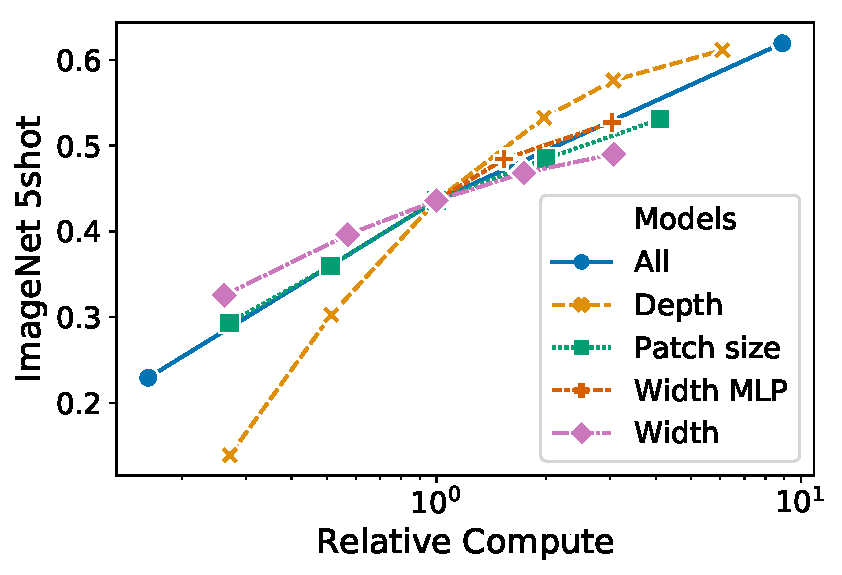
\includegraphics[width=\textwidth]{images/compute_analysis/transformer_shape_imagenet_5shot.pdf}
\end{center}
\end{minipage}\quad
\begin{minipage}[t]{0.47\textwidth}
\begin{center}
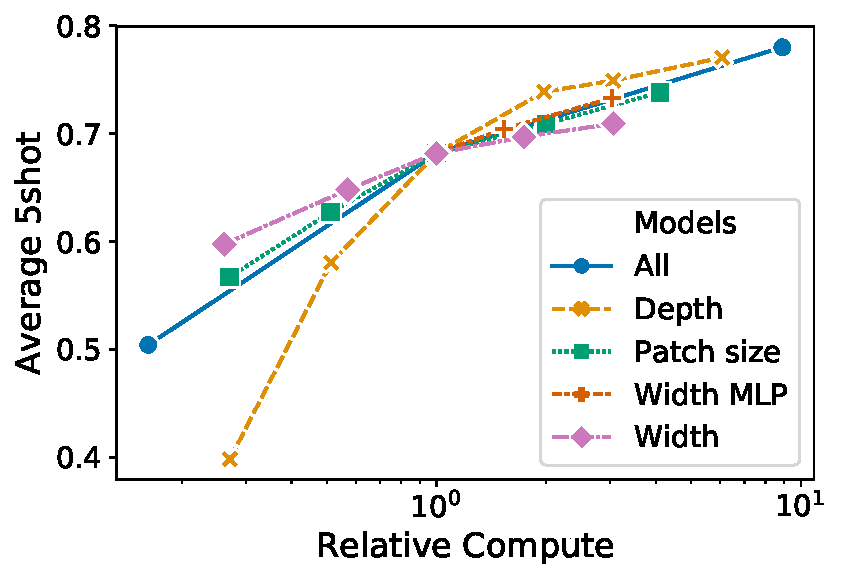
\includegraphics[width=\textwidth]{images/compute_analysis/transformer_shape_average_5shot.pdf}
\end{center}
\label{fig:scaling_transformers_average}
\end{minipage}
\caption{Scaling different model dimensions of the \oursfull.}
\label{fig:scaling_transformers}
\end{figure}

We ran ablations on scaling different dimensions of the Transformer architecture to find out which are best suited for scaling to very large models. Figure~\ref{fig:scaling_transformers} shows 5-shot performance on \imagenet for different configurations. All configurations are based on a \oursabbrv model with $8$ layers, $D=1024$, $D_{MLP}=2048$ and a patch size of $32$, the intersection of all lines. We can see that scaling the depth results in the biggest improvements which are clearly visible up until 64 layers. However, diminishing returns are already visible after 16 layers. Interestingly, scaling the width of the network seems to result in the smallest changes. Decreasing the patch size and thus increasing the effective sequence length shows surprisingly robust improvements without introducing parameters. These findings suggest that compute might be a better predictor of performance than the number of parameters, and that scaling should emphasize depth over width if any. Overall, we find that scaling all dimensions proportionally results in robust improvements.

\begin{figure}[t]
\begin{center}
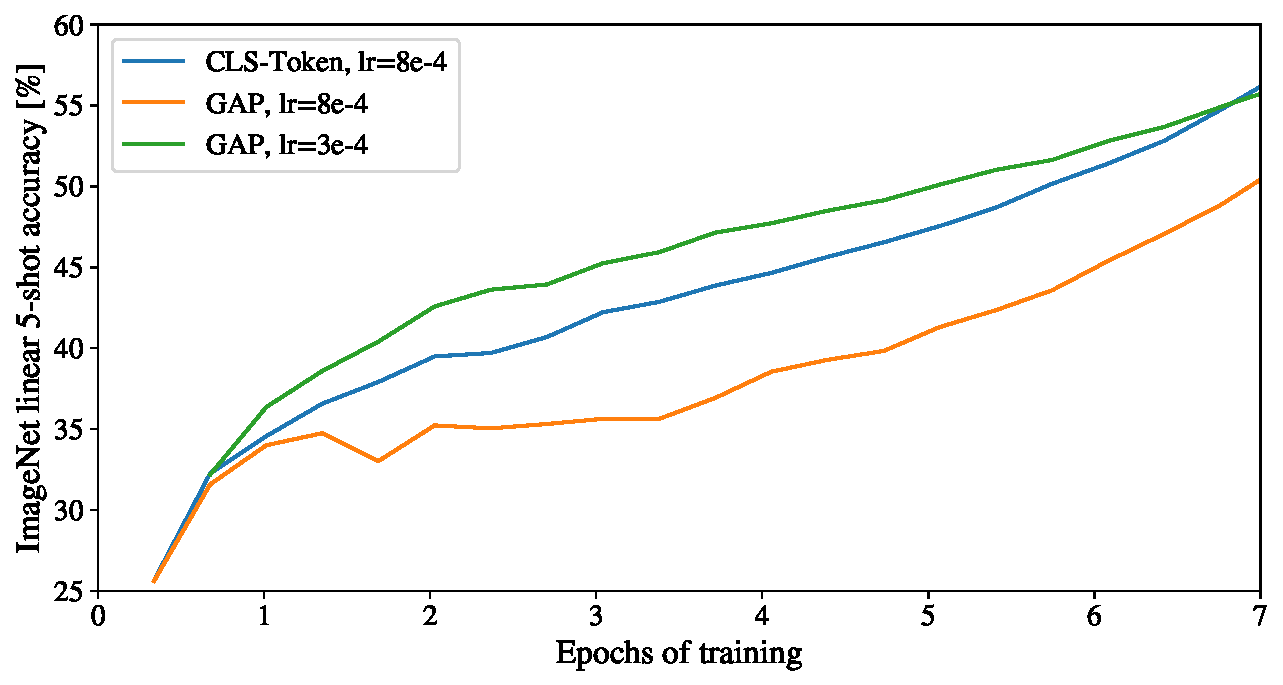
\includegraphics[width=0.7\textwidth]{images/head_tokens}
\end{center}
\caption{Comparison of class-token and global average pooling classifiers. Both work similarly well, but require different learning-rates.}
\label{fig:head_tokens}
\end{figure}

\subsection{Head Type and \texttt{class} token}
\label{app:head_types}
In order to stay as close as possible to the original Transformer model, we made use of an additional \texttt{[class]} token, which is taken as image representation. The output of this token is then transformed into a class prediction via a small multi-layer perceptron (MLP) with $\tanh$ as non-linearity in the single hidden layer.

This design is inherited from the Transformer model for text, and we use it throughout the main paper.
An initial attempt at using only image-patch embeddings, globally average-pooling (GAP) them, followed by a linear classifier---just like ResNet's final feature map---performed very poorly.
However, we found that this is neither due to the extra token, nor to the GAP operation. Instead, the difference in performance is fully explained by the requirement for a different learning-rate, see Figure~\ref{fig:head_tokens}.

\subsection{Positional Embedding}
\label{app:pos_emb}

We ran ablations on different ways of encoding spatial information using positional embedding. We tried the following cases:
\begin{itemize}
    \item Providing no positional information: Considering the inputs as a \emph{bag of patches}.
    \item 1-dimensional positional embedding: Considering the inputs as a sequence of patches in the raster order (default across all other experiments in this paper).
    \item 2-dimensional positional embedding: Considering the inputs as a grid of patches in two dimensions. In this case, two sets of embeddings are learned, each for one of the axes, $X$-embedding, and $Y$-embedding, each with size $D/2$. Then, based on the coordinate on the path in the input, we concatenate the $X$ and $Y$ embedding to get the final positional embedding for that patch.
    \item Relative positional embeddings:  Considering the relative distance between patches to encode the spatial information as instead of their absolute position. To do so, we use 1-dimensional Relative Attention, in which we define the relative distance all possible pairs of patches. Thus, for every given pair (one as query, and the other as key/value in the attention mechanism), we have an offset $p_{q}-p_{k}$, where each offset is associated with an embedding. Then, we simply run extra attention, where we use the original query (the content of query), but use relative positional embeddings as keys. We then use the logits from the relative attention as a bias term and add it to the logits of the main attention (content-based attention) before applying the softmax. 
\end{itemize}



\begin{table}[t]
\centering
\begin{tabular}{l c c c}
\toprule
Pos. Emb. & Default/Stem & Every Layer & Every Layer-Shared \\
\midrule
No Pos. Emb. & 0.61382  & N/A & N/A \\
1-D Pos. Emb. & 0.64206 & 0.63964 & 0.64292 \\
2-D Pos. Emb. &  0.64001 & 0.64046  & 0.64022 \\
Rel. Pos. Emb. & 0.64032 & N/A & N/A \\
\bottomrule
\end{tabular}
\caption{Results of the ablation study on positional embeddings with \oursabbrv-B/16 model evaluated on \imagenet 5-shot linear.}
\label{tbl:pos_emb_abblation}
\end{table}

\begin{figure}[t]
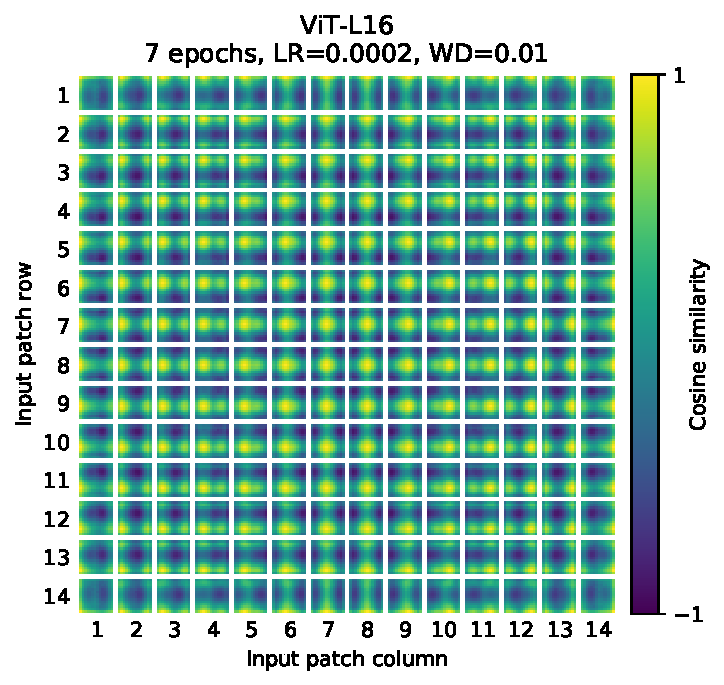
\includegraphics[height=1.8in,trim={0in 0in 0.65in 0in},clip]{images/visualizations/20200930_position_embeddings_16490619_1.pdf}
\hfill
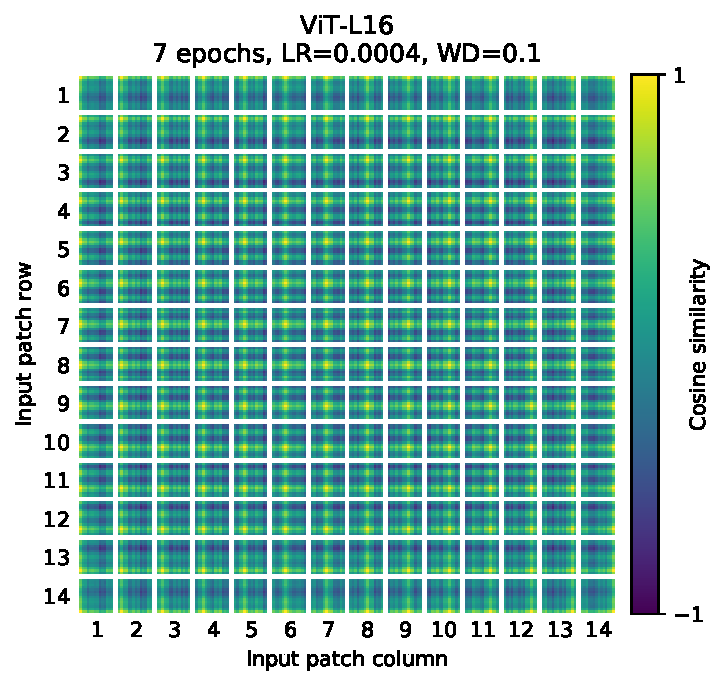
\includegraphics[height=1.8in,trim={0in 0in 0.65in 0in},clip]{images/visualizations/20200930_position_embeddings_17192124_1.pdf}
\hfill
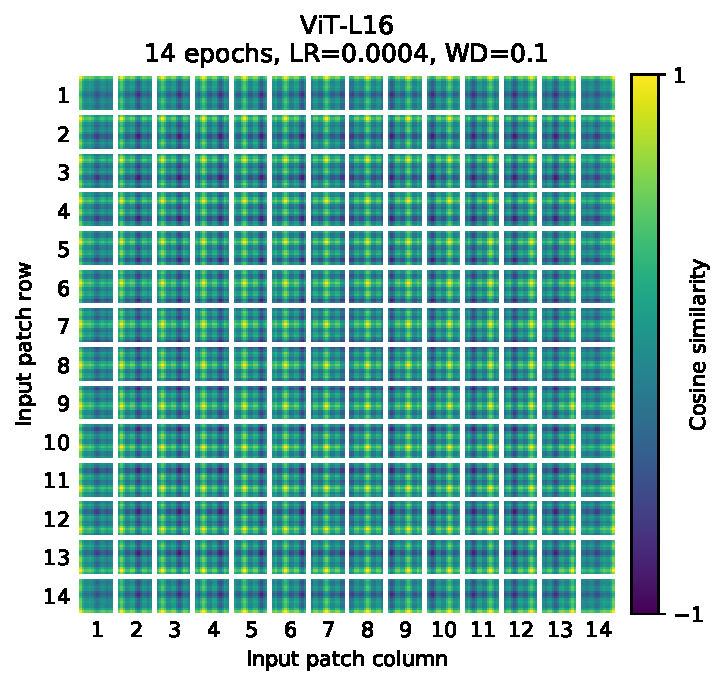
\includegraphics[height=1.8in,trim={0in 0in 0in 0in},clip]{images/visualizations/20200930_position_embeddings_17192217_1.pdf}
\caption{Position embeddings of models trained with different hyperparameters.}
\label{fig:position_embedding_comparison}
\end{figure}

In addition to different ways of encoding spatial information, we also tried different ways of incorporating this information in our model. For the 1-dimensional and 2-dimensional positional embeddings, we tried three different cases: (1) add positional embeddings to the inputs right after the stem of them model and before feeding the inputs to the Transformer encoder (default across all other experiments in this paper); (2) learn and add positional embeddings to the inputs at the beginning of each layer; (3) add a learned positional embeddings to the inputs at the beginning of each layer (shared between layers).

Table~\ref{tbl:pos_emb_abblation} summarizes the results from this ablation study on a \oursabbrv-B/16 model. As we can see, while there is a large gap between the performances of the model with no positional embedding and models with positional embedding, there is little to no difference between different ways of encoding positional information. We speculate that since our Transformer encoder operates on patch-level inputs, as opposed to pixel-level, the differences in how to encode spatial information is less important. More precisely, in patch-level inputs, the spatial dimensions are much smaller than the original pixel-level inputs, e.g., $14\times14$ as opposed to $224\times224$, and learning to represent the spatial relations in this resolution is equally easy for these different positional encoding strategies.
Even so, the specific pattern of position embedding similarity learned by the network depends on the training hyperparameters (Figure~\ref{fig:position_embedding_comparison}).

\begin{figure}[h]
\begin{center}
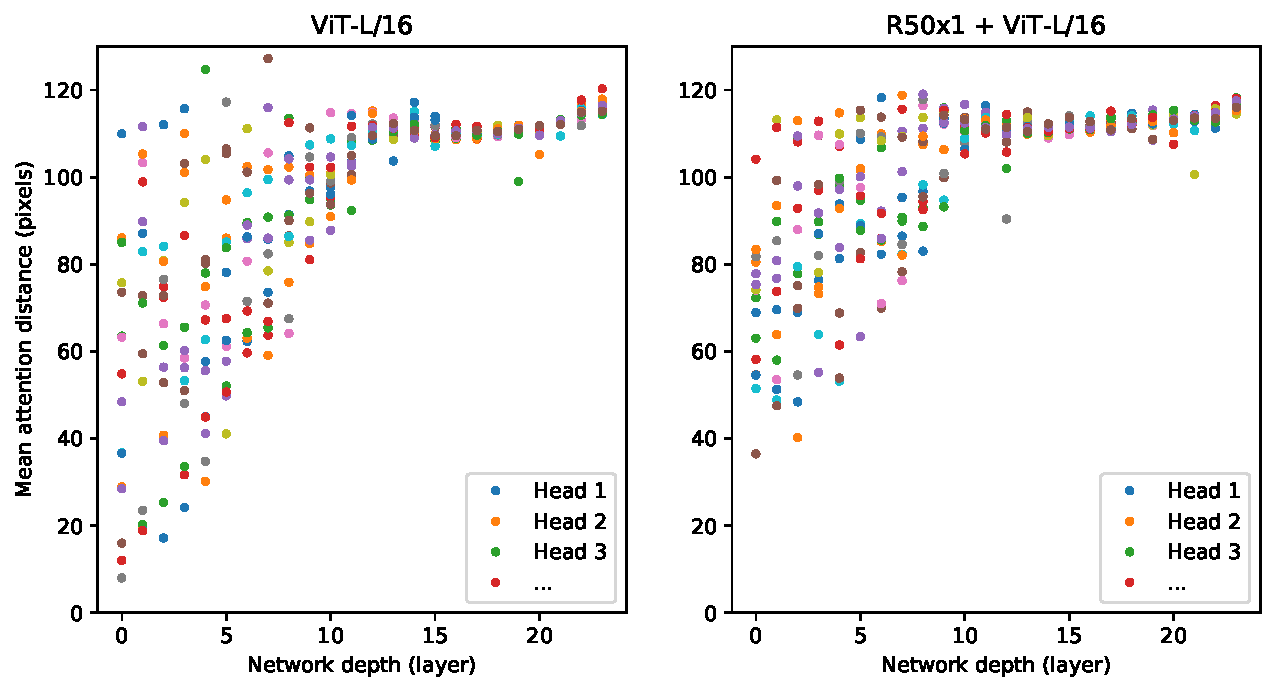
\includegraphics[height=2.5in]{images/visualizations/20201001_attention_distance_by_depth.pdf}
\end{center}
\caption{Size of attended area by head and network depth. Attention distance was computed for 128 example images by averaging the distance between the query pixel and all other pixels, weighted by the attention weight. Each dot shows the mean attention distance across images for one of 16 heads at one layer. Image width is 224 pixels.}
\label{fig:attention_distance}
\end{figure}

\subsection{Empirical Computational Costs}
\label{sec:empirical_computation}

We are also interested in real-world speed of the architectures on our hardware, which is not always well predicted by theoretical FLOPs due to details like lane widths and cache sizes.
For this purpose, we perform timing of inference speed for the main models of interest, on a TPUv3 accelerator; the difference between inference and backprop speed is a constant model-independent factor.

Figure~\ref{fig:real_time}~(left) shows how many images one core can handle per second, across various input sizes.
Every single point refers to the peak performance measured across a wide range of batch-sizes.
As can be seen, the theoretical bi-quadratic scaling of ViT with image size only barely starts happening for the largest models at the largest resolutions.

Another quantity of interest is the largest batch-size each model can fit onto a core, larger being better for scaling to large datasets.
Figure~\ref{fig:real_time}~(right) shows this quantity for the same set of models.
This shows that large ViT models have a clear advantage in terms of memory-efficiency over ResNet models.

\begin{figure}[h]
\begin{center}
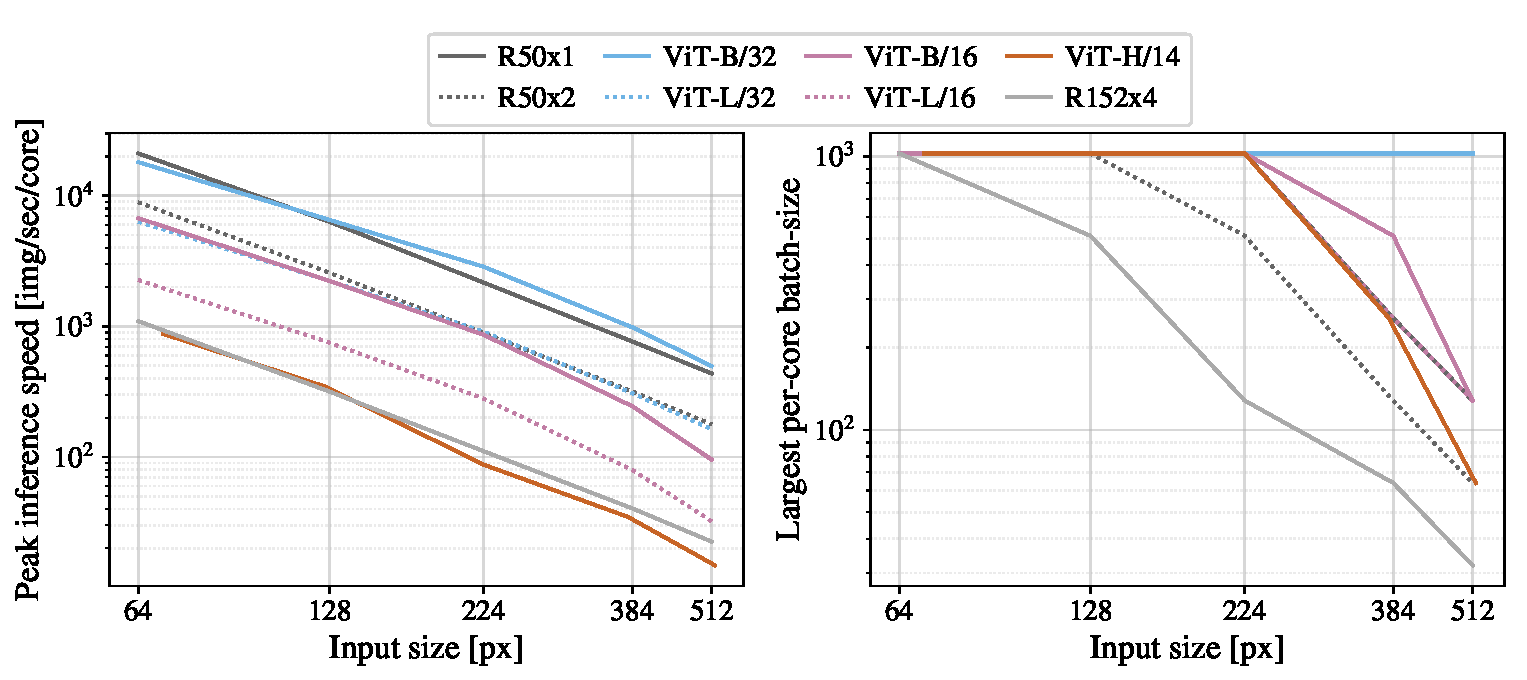
\includegraphics[width=0.92\textwidth]{images/img_sec_core}
\end{center}
\caption{\textbf{Left:} Real wall-clock timings of various architectures across input sizes. ViT models have speed comparable to similar ResNets.
\textbf{Right}: Largest per-core batch-size fitting on device with various architectures across input sizes. ViT models are clearly more memory-efficient.}
\label{fig:real_time}
\end{figure}

\subsection{Axial Attention}
Axial Attention~\citep{huang2020ccnet,ho2019-axialattention} is a simple, yet effective technique to run self-attention on large inputs that are organized as multidimensional tensors. The general idea of axial attention is to perform multiple attention operations, each along a single axis of the input tensor, instead of applying 1-dimensional attention to the flattened version of the input. In axial attention, each attention mixes information along a particular axis, while keeping information along the other axes independent. 
Along this line, \citet{wang2020axial} proposed the AxialResNet model in which all the convolutions with kernel size $3\times3$ in a ResNet50 are replaced by axial self-attention, i.e. a row and column attention, augmented by relative positional encoding. 
We have implemented AxialResNet as a baseline model.\footnote{Our implementation is based on the open-sourced PyTorch implementation in \url{https://github.com/csrhddlam/axial-deeplab}. In our experiments, we reproduced the scores reported in~\citep{wang2020axial} in terms of accuracy, however, our implementation, similar to the open-source implementation, is very slow on TPUs.
Therefore, we were not able to use it for extensive large-scale experiments.
These may be unlocked by a carefully optimized implementation.}.

Moreover, we have modified \oursabbrv to process inputs in the 2-dimensional shape, instead of a 1-dimensional sequence of patches, and incorporate Axial Transformer blocks, in which instead of a self-attention followed by an MLP, we have a a row-self-attention plus an MLP followed by a column-self-attention plus an MLP. 
\begin{figure}[h]
    \centering
    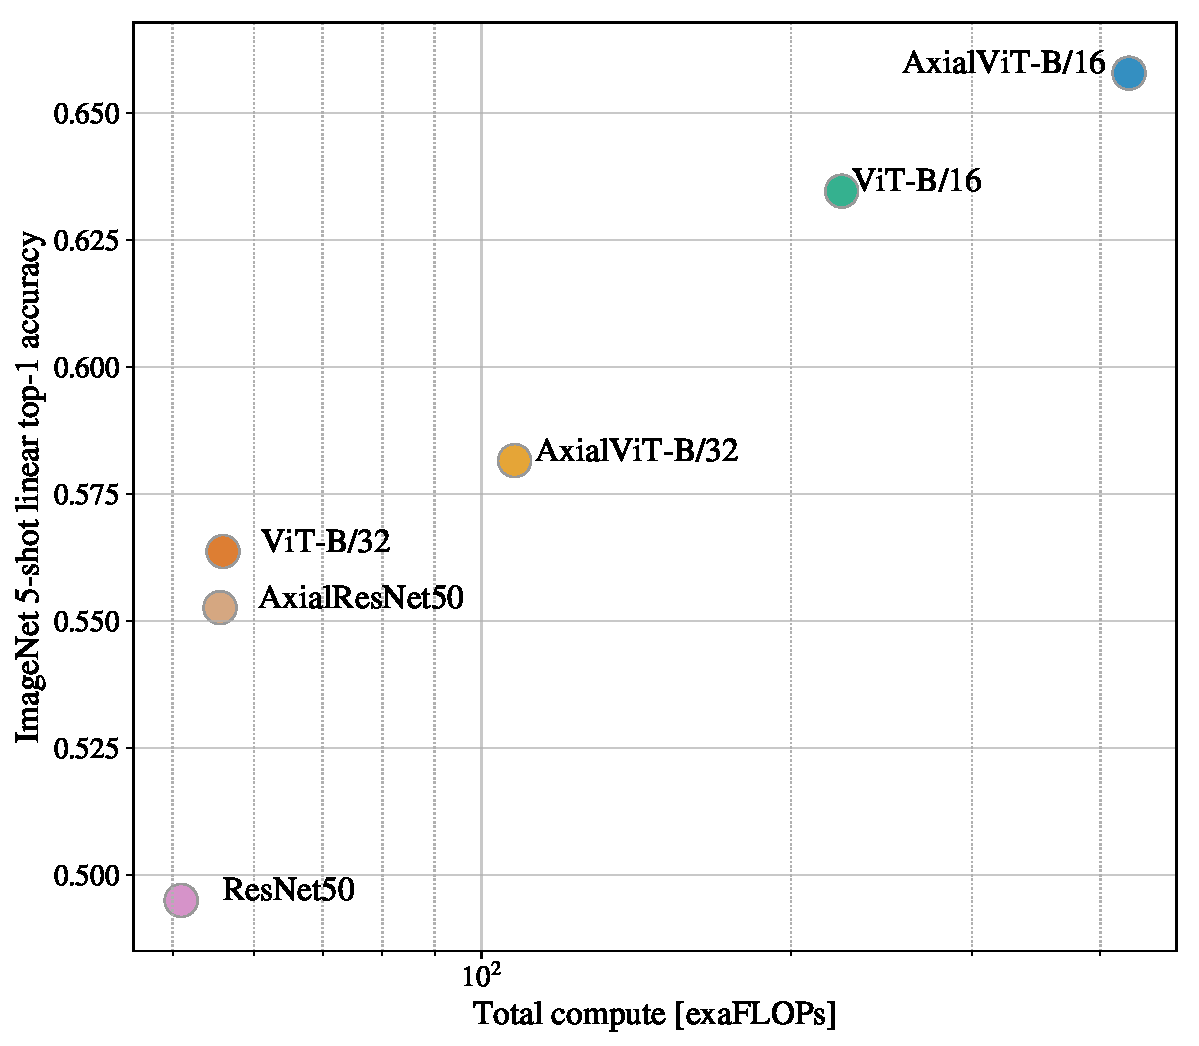
\includegraphics[width=0.45\textwidth]{images/compute_analysis/axial_flop.pdf}
    \hspace{10pt}
    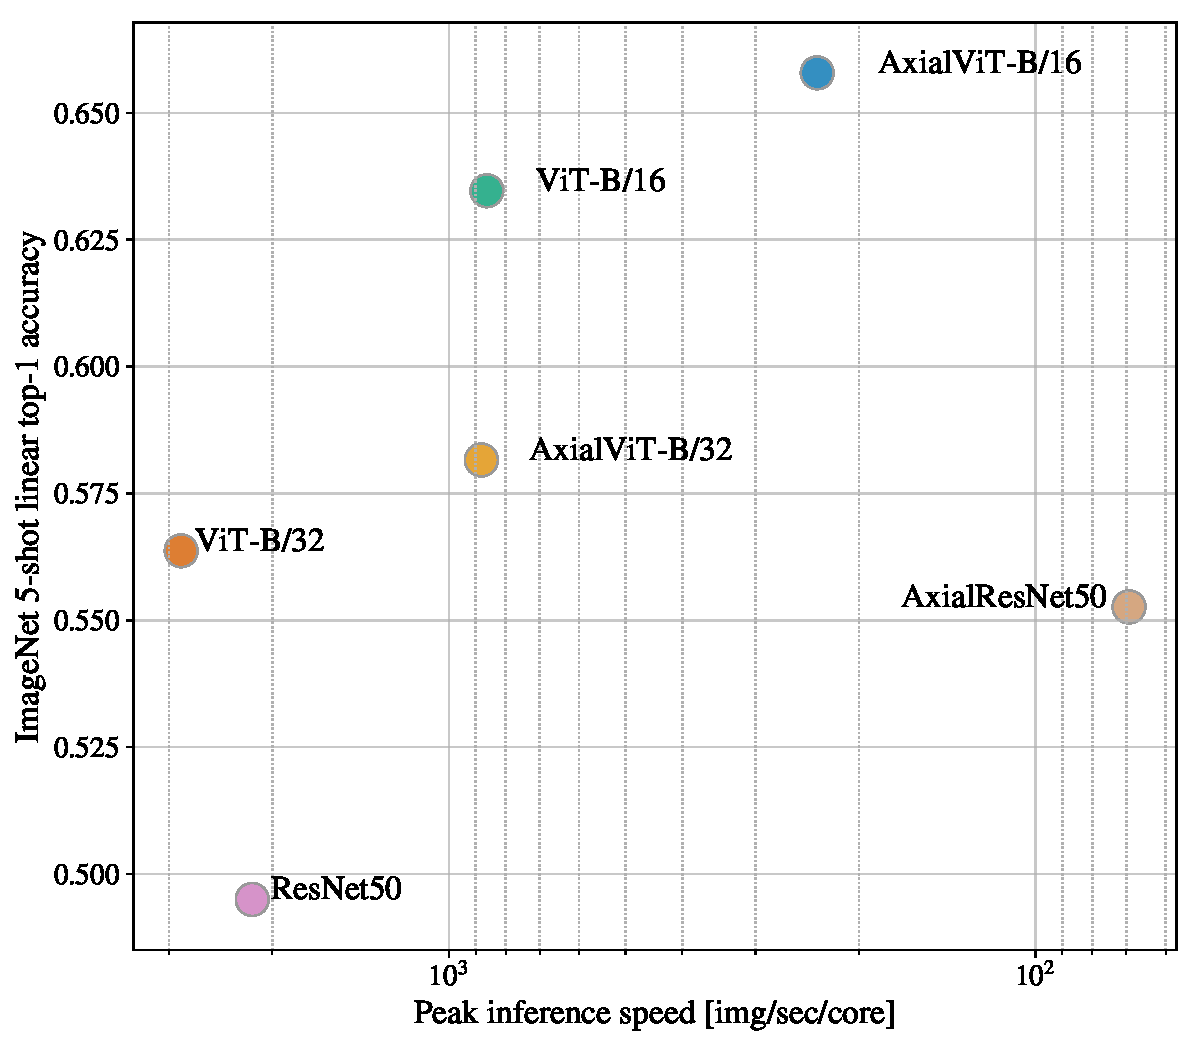
\includegraphics[width=0.45\textwidth]{images/compute_analysis/axial_img_sec_core.pdf}
    \caption{Performance of Axial-Attention based models, in terms of top-1 accuracy on ImageNet 5-shot linear, versus their speed in terms of number of FLOPs (\textbf{left}) and inference time (\textbf{left}).}
    \label{fig:axial_compute_performance}
\end{figure}

Figure~\ref{fig:axial_compute_performance}, present the performance of Axial ResNet, Axial-\oursabbrv-B/32 and Axial-\oursabbrv-B/16 on \imagenet 5shot linear, when pretrained on JFT dataset, verses the pretraining compute, both in terms of number of FLOPs and inference time (example per seconds). As we can see, both 
Axial-\oursabbrv-B/32 and Axial-\oursabbrv-B/16 do better than their \oursabbrv-B counterpart in terms of performance, but it comes at the cost of more compute. This is because in Axial-\oursabbrv models, each Transformer block with global self-attention is replaced by two Axial Transformer blocks, one with row and one with column self-attention and although the sequence length that self-attention operates on is smaller in axial case, there is a extra MLP per Axial-\oursabbrv block.  
For the AxialResNet, although it looks reasonable in terms of accuracy/compute trade-off (Figure~\ref{fig:axial_compute_performance}, left), the naive implementation is extremely slow on TPUs (Figure~\ref{fig:axial_compute_performance}, right).


 
\subsection{Attention Distance}
\label{sec:appendix_attention_distance}

To understand how \oursabbrv uses self-attention to integrate information across the image, we analyzed the average distance spanned by attention weights at different layers (Figure~\ref{fig:attention_distance}). This ``attention distance'' is analogous to receptive field size in CNNs. Average attention distance is highly variable across heads in lower layers, with some heads attending to much of the image, while others attend to small regions at or near the query location. As depth increases, attention distance increases for all heads. In the second half of the network, most heads attend widely across tokens.

\subsection{Attention Maps}
To compute maps of the attention from the output token to the input space (Figures~\ref{fig:selected_attention_examples} and \ref{fig:batch_attention_examples}), we used Attention Rollout \citep{abnar2020quantifying}. Briefly, we averaged attention weights of \oursabbrv-L/16 across all heads and then recursively multiplied the weight matrices of all layers. This accounts for the mixing of attention across tokens through all layers.

\begin{figure}[h]
\begin{center}
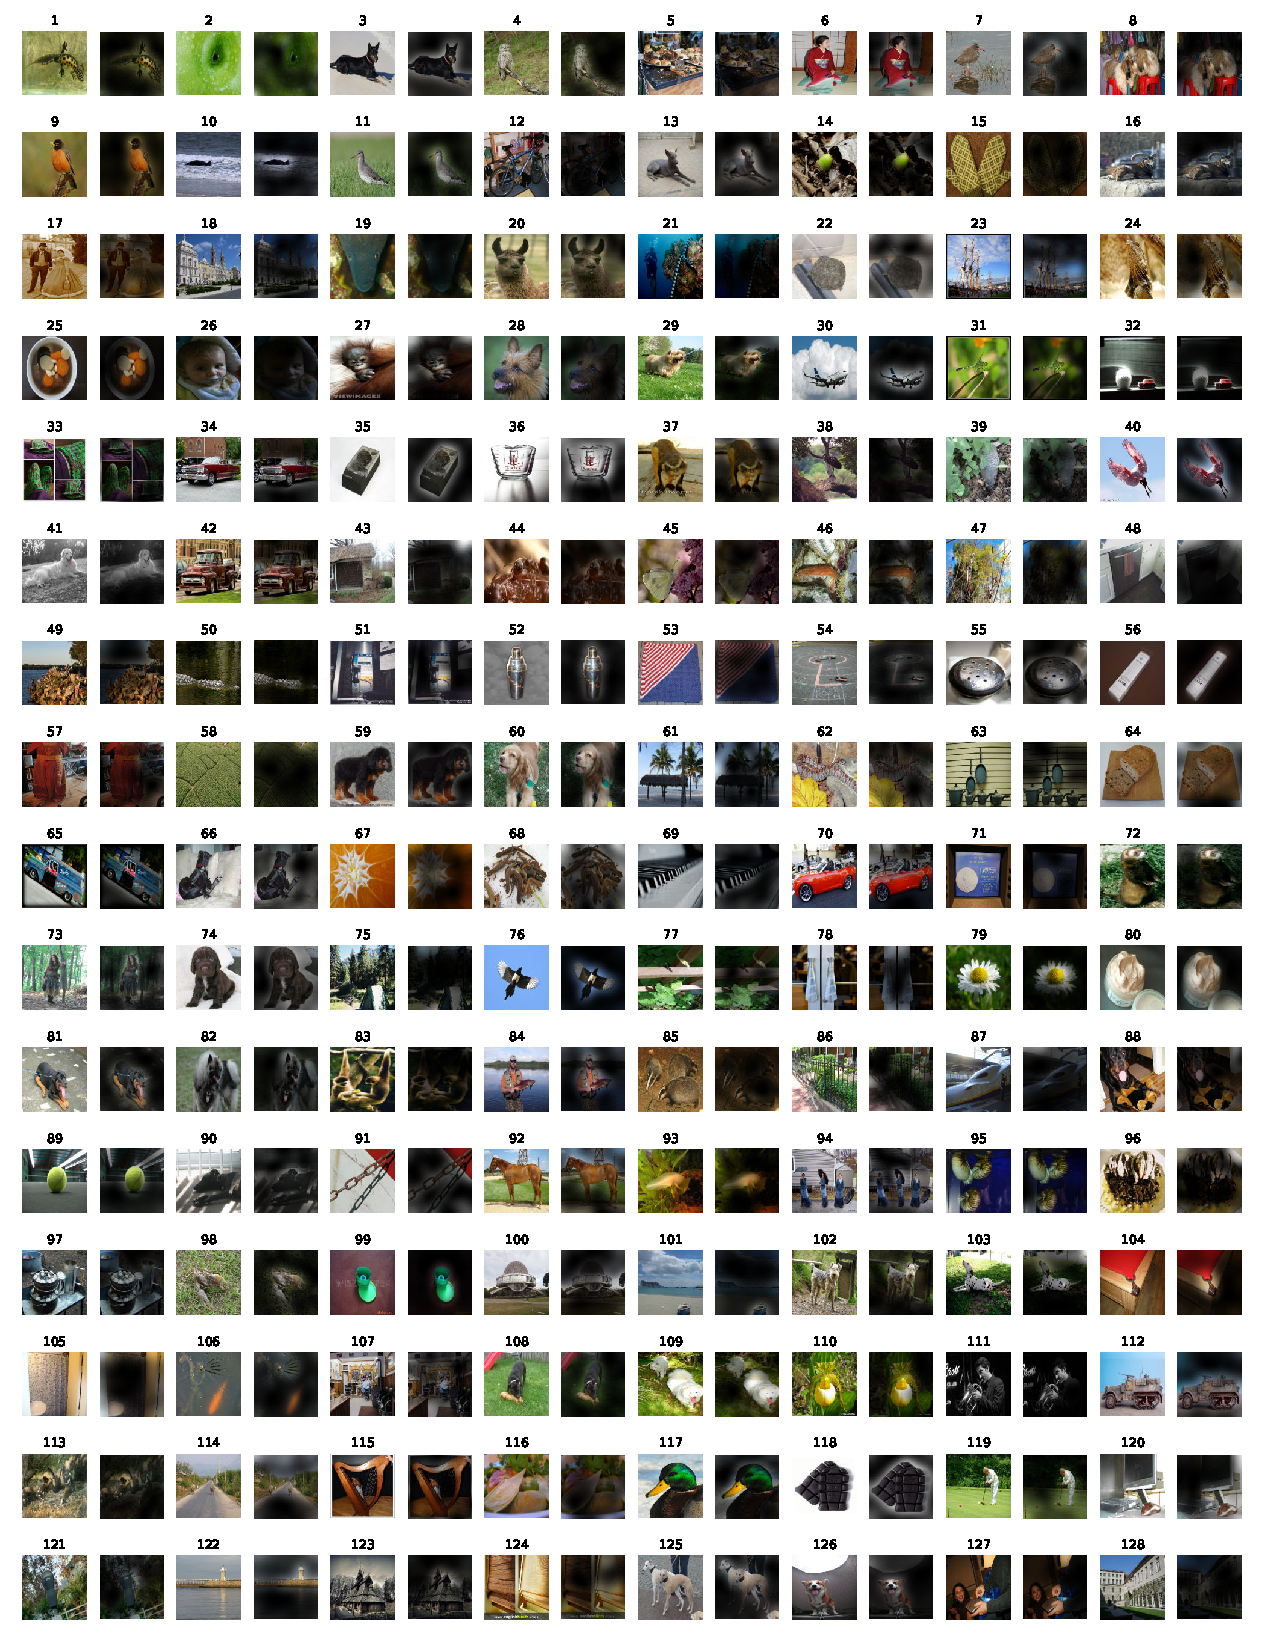
\includegraphics[width=\textwidth]{images/visualizations/20201002_batch_attention_examples_compressed.pdf}
\end{center}
\caption{Further example attention maps as in Figure~\ref{fig:selected_attention_examples} (random selection).}
\label{fig:batch_attention_examples}
\end{figure}

\subsection{ObjectNet Results}
We also evaluate our flagship ViT-H/14 model on the ObjectNet benchmark following the evaluation setup in~\cite{kolesnikov2020-bit}, resulting in 82.1\% top-5 accuracy and 61.7\% top-1 accuracy.

\subsection{VTAB Breakdown}
Table~\ref{tab:vtab_tasks} shows the scores attained on each of the VTAB-1k tasks.

\begin{table}[ht]
\centering
\caption{
Breakdown of VTAB-1k performance across tasks.
}


\fontsize{7pt}{7pt}\selectfont
\newcolumntype{C}{>{\centering\arraybackslash}X}
\setlength{\tabcolsep}{0pt}
\setlength{\extrarowheight}{5pt}
\renewcommand{\arraystretch}{0.75}
\begin{tabularx}{\linewidth}{p{10pt}p{1.6cm}!{\color{lightgray}\vline} CCCCCCC!{\color{lightgray}\vline}CCCC!{\color{lightgray}\vline}CCCCCCCC!{\color{lightgray}\vline}C}
\toprule
 &
 & \rotatebox{90}{\raisebox{0.5pt}{\tikz\fill[natural] (0,0) circle (.5ex);} Caltech101}
 & \rotatebox{90}{\raisebox{0.5pt}{\tikz\fill[natural] (0,0) circle (.5ex);} CIFAR-100}
 & \rotatebox{90}{\raisebox{0.5pt}{\tikz\fill[natural] (0,0) circle (.5ex);} DTD}
 & \rotatebox{90}{\raisebox{0.5pt}{\tikz\fill[natural] (0,0) circle (.5ex);} Flowers102}
 & \rotatebox{90}{\raisebox{0.5pt}{\tikz\fill[natural] (0,0) circle (.5ex);} Pets}
 & \rotatebox{90}{\raisebox{0.5pt}{\tikz\fill[natural] (0,0) circle (.5ex);} Sun397}
 & \rotatebox{90}{\raisebox{0.5pt}{\tikz\fill[natural] (0,0) circle (.5ex);} SVHN}
 & \rotatebox{90}{\raisebox{0.5pt}{\tikz\fill[specialized] (0,0) circle (.5ex);} Camelyon}
 & \rotatebox{90}{\raisebox{0.5pt}{\tikz\fill[specialized] (0,0) circle (.5ex);} EuroSAT}
 & \rotatebox{90}{\raisebox{0.5pt}{\tikz\fill[specialized] (0,0) circle (.5ex);} Resisc45}
 & \rotatebox{90}{\raisebox{0.5pt}{\tikz\fill[specialized] (0,0) circle (.5ex);} Retinopathy}
 & \rotatebox{90}{\raisebox{0.5pt}{\tikz\fill[structured] (0,0) circle (.5ex);} Clevr-Count}
 & \rotatebox{90}{\raisebox{0.5pt}{\tikz\fill[structured] (0,0) circle (.5ex);} Clevr-Dist}
 & \rotatebox{90}{\raisebox{0.5pt}{\tikz\fill[structured] (0,0) circle (.5ex);} DMLab}
 & \rotatebox{90}{\raisebox{0.5pt}{\tikz\fill[structured] (0,0) circle (.5ex);} dSpr-Loc}
 & \rotatebox{90}{\raisebox{0.5pt}{\tikz\fill[structured] (0,0) circle (.5ex);} dSpr-Ori}
 & \rotatebox{90}{\raisebox{0.5pt}{\tikz\fill[structured] (0,0) circle (.5ex);} KITTI-Dist}
 & \rotatebox{90}{\raisebox{0.5pt}{\tikz\fill[structured] (0,0) circle (.5ex);} sNORB-Azim}
 & \rotatebox{90}{\raisebox{0.5pt}{\tikz\fill[structured] (0,0) circle (.5ex);} sNORB-Elev}
 & \rotatebox{90}{\raisebox{0.5pt}{\tikz\fill[all] (0,0) circle (.5ex);} Mean} \\
\midrule

& \oursabbrv{}-H/14 (JFT) & 95.3 & 85.5 & 75.2 & 99.7 & 97.2 & 65.0 & 88.9 & 83.3 & 96.7 & 91.4 & 76.6 & 91.7 & 63.8 & 53.1 & 79.4 & 63.3 & 84.5 & 33.2 & 51.2 & 77.6  \\

& \oursabbrv{}-L/16 (JFT) & 95.4 & 81.9 & 74.3 & 99.7 & 96.7 & 63.5 & 87.4 & 83.6 & 96.5 & 89.7 & 77.1 & 86.4 & 63.1 & 49.7 & 74.5 & 60.5 & 82.2 & 36.2 & 51.1 & 76.3  \\

& \oursabbrv{}-L/16 (I21k) & 90.8 & 84.1 & 74.1 & 99.3 & 92.7 & 61.0 & 80.9 & 82.5 & 95.6 & 85.2 & 75.3 & 70.3 & 56.1 & 41.9 & 74.7 & 64.9 & 79.9 & 30.5 & 41.7 & 72.7  \\

\bottomrule
\end{tabularx}

\label{tab:vtab_tasks}
\end{table}